\documentclass[a4paper,12pt]{article}
\usepackage{mathtools,amsfonts,amssymb,amsmath, bm,commath,multicol}
\usepackage{algorithmicx, tkz-graph, algorithm, fancyhdr, minted, pgfplots}
\usepackage{textgreek}
\usepackage{graphicx}
\usepackage{fancyvrb}
\usepackage{hyperref}

\usepackage[noend]{algpseudocode}

\DefineVerbatimEnvironment{juliaout}{Verbatim}{}
\DefineVerbatimEnvironment{juliacode}{Verbatim}{fontshape=sl, fontsize=\tiny}
\DefineVerbatimEnvironment{juliaterm}{Verbatim}{}


\begin{document}

\section*{5}
This question is most easily explained by overlaying the PDF's of the two classes:

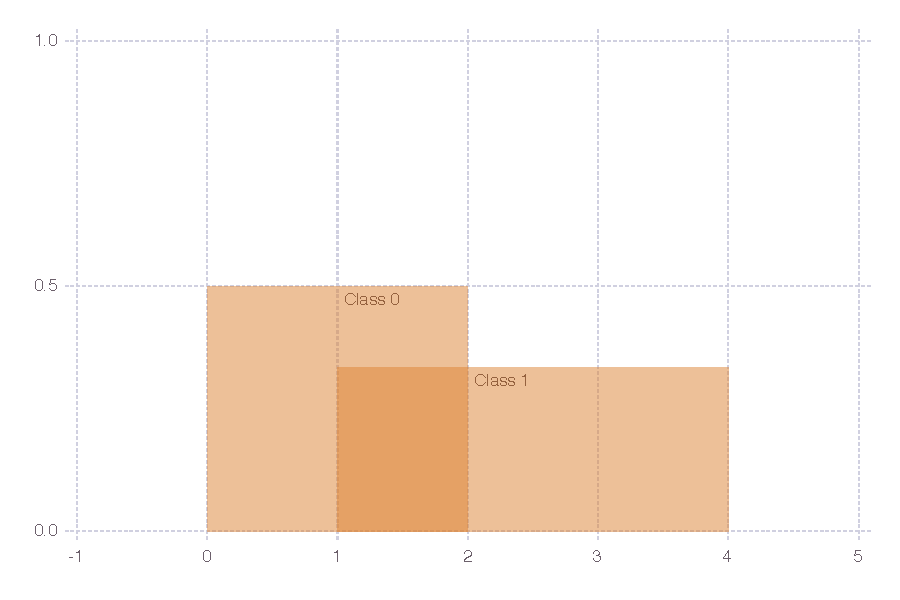
\includegraphics[width=\linewidth]{figures/weave-test_1_1.pdf}



The bayes classifier is very simple, from 0-2, pick 0, while from 2-4, you pick 1. The Bayes risk is simply the overlapping area in the graph of the two PDF's. When values are between 1-2, there is a risk of 2/5. This is obtained by summing all the possibilities to obtain our marginilizing constant, and then taking the density of class 1 over the area (1/3):

\begin{align*}
\frac{\frac{1}{3}}{\frac{1}{3} + \frac{1}{2}} &= \frac{2}{5}
\end{align*}
%
To compute the asymptotic 1-nearest neighbor risk, we imagine we have infinity observations. The nearest neighbor will therefore be picked out of a bag at random. In the area where the two classes overlap, there is a 3/5 chance of getting class 0 and a 2/5 chance of getting class 1. The risk is the expected loss, in the descrete case we sum over all the possiblities, multiplied by their probability, to get the expectation:

\begin{align*}
\mathbb{E}(L_{1-nn}) &= \sum_x L(x)p(x) \\
\mathbb{E}(L_{1-nn}) &= \sum_{x \in L(x) \neq 0 } L(x)p(x) \\
\mathbb{E}(L_{1-nn}) &= 1*\eta(x)(1-\eta(x)) + 1*(1-\eta(x))\eta(x) \\
\mathbb{E}(L_{1-nn}) &= 2\eta(x)(1-\eta(x)) \\
\mathbb{E}(L_{1-nn}) &= 2(\frac{2}{5})(\frac{3}{5}) \\
\mathbb{E}(L_{1-nn}) &= \frac{12}{25}
\end{align*}

\section*{6}


\section*{7}


\end{document}